\section{Guida all'installazione}

Prima di essere in grado di eseguire il programma, è necessario eseguire il file \texttt{risorse.bat} contenuto nella cartella Risorse. 


Una volta eseguito il file, si aprirà una pagina ti Powershell e seguirà un download.

\begin{figure}[h!]
    \centering
    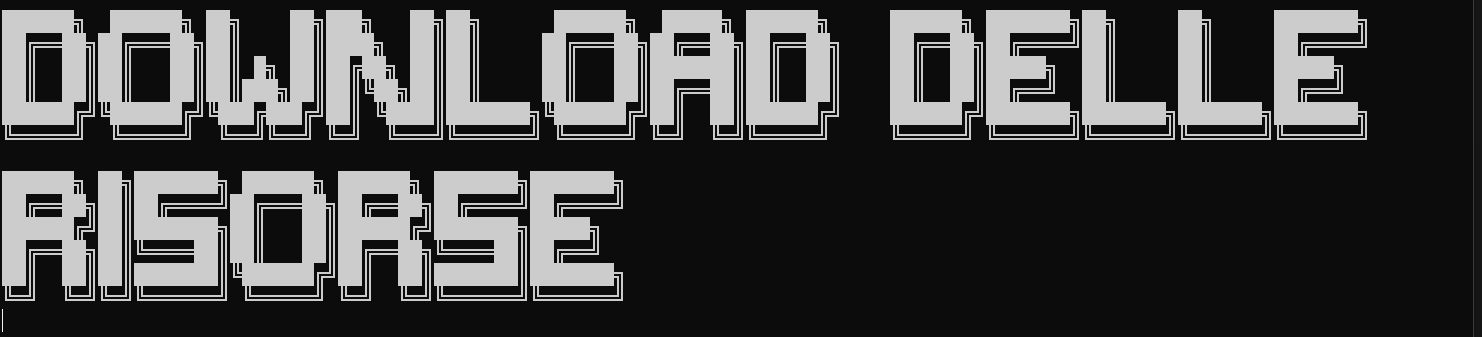
\includegraphics[width= 0.5\textwidth]{images/nuova docs.png}
    \caption{Schermatta di download}
\end{figure}

Al termine del download del file compresso delle risorse, verranno estratti i file necessari per l'esecuzione del programma.



Per il progetto in questione è necessario installare il Java Developer Kit (JDK) nella versione 22.0.1 e il software di gestione del database MySQL nella sua versione 8.0.39. 

La prima scheda di installazione che apparirà è quella del JDK. 

Verrà chiesto se si vuole eseguire l'installazione del JDK tramite permessi di amministratore, cliccare su \underline{Sì}.

\subsection{Installazione JDK}

Una volta confermata l'esecuzione come amministratore, si procederà all'installazione del JDK.

\begin{figure}[h!]
    \centering
    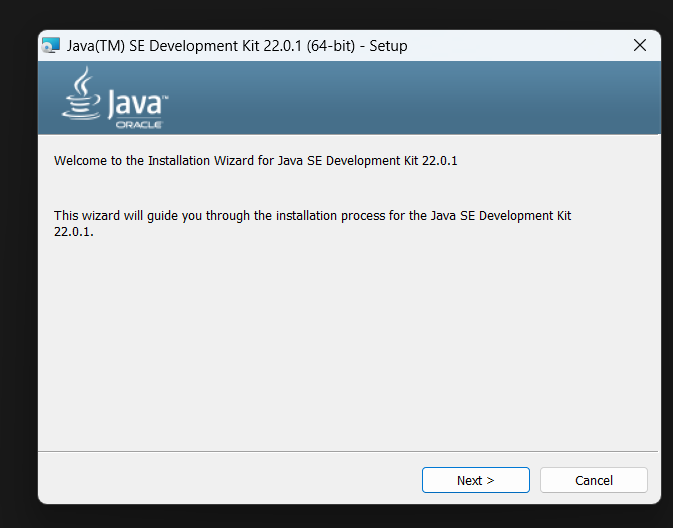
\includegraphics[width= 0.5\textwidth]{images/installazione java.png}
\end{figure}

Cliccare su \textbf{Avanti},nuovamente \textbf{Avanti} e infine, nel caso in cui l'installazione sia andata a buon fine, si dovràò cliccare sul tasto \textbf{Chiudi}.

\subsection{Variabili di ambiente}

è consigliato creare una variabile di ambiente per il JDK. Per farlo, si dovrà cercare la voce \textbf{variabili di ambiente} nella barra di ricerca di Windows e cliccare su {Modifica le variabili di ambiente per il tuo account}.

Successivamente si dovrà cliccare sul pulsante \textbf{Variabili di ambiente} e si aprirà una schermata con le variabili di ambiente. 



\begin{figure}[h!]
    \centering
    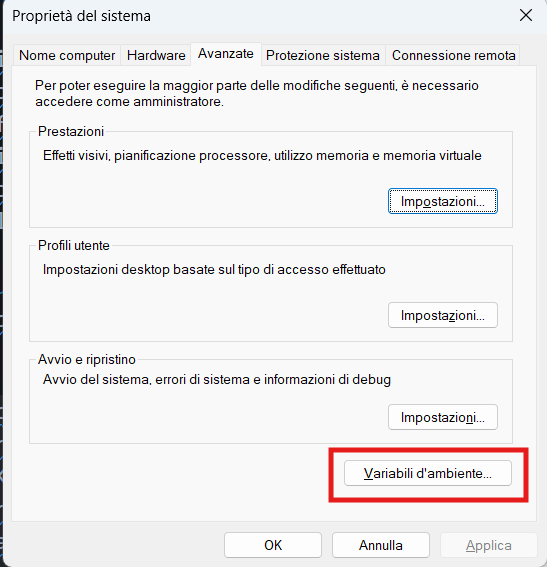
\includegraphics[width= 0.5\textwidth]{images/variabili ambienti.png}
    \caption{Schermata delle variabili di ambiente}
\end{figure}

Nella schermata, si dovra cliccare sulla variabile \texttt{PATH} e modificarla in modo da aggiungere il percorso del JDK, inserendo il percorso in cui è stato installato il JDK.

Una volta completata l'installazione del JDK, si procederà automaticamente con l'installazione del MySQL.



\subsection{Installazione MySQL}

Anche qui sarà necessario fornire i permessi di amministratore, cliccare dunque su \underline{Sì}.

\subsection{Schermata iniziale}

Dopodiché si aprirà la schermata di installazione di MySQL.

\begin{figure}[h!]
    \centering
    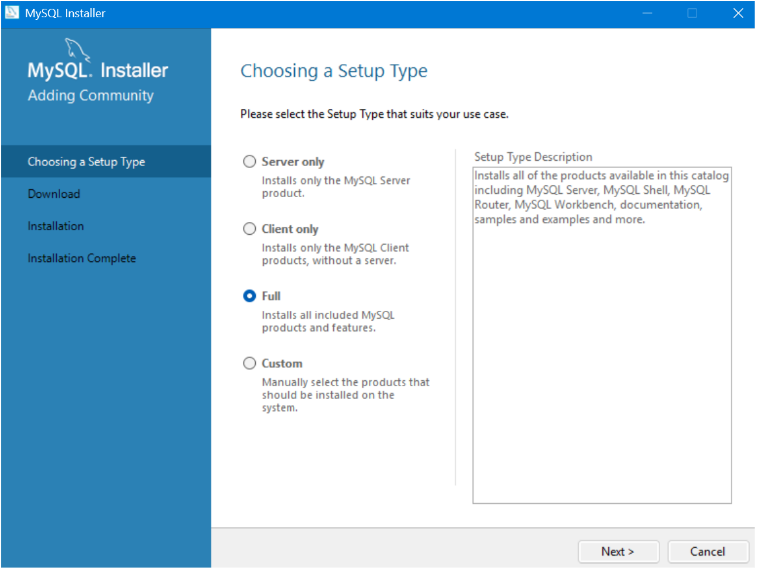
\includegraphics[width= 0.5\textwidth]{images/inizio mysql.png}
    \caption{Scelta del setup}
\end{figure}

Selezionare il tipo di setup \textbf{Full} e cliccare su \textbf{Next}. Tale scelta permetterà di installare tutti i componenti necessari per l'esecuzione del programma.

\subsection{Download dei file}

Si passerà alla schermata di download dei file necessari per l'installazione, cliccare su \textbf{Execute}. 

\begin{tcolorbox}[  colback=white!5!white, colframe=gray, title={Avvertenza} ]
    
    
    Tale schermata potrebbe richiedere un po' di tempo per il download dei file, a seconda della velocità della connessione internet. 
\end{tcolorbox}
    
Dopo aver scaricato i file, si dovrà cliccare nuovamente su \textbf{Execute}.

\begin{figure}[h!]
    \centering
    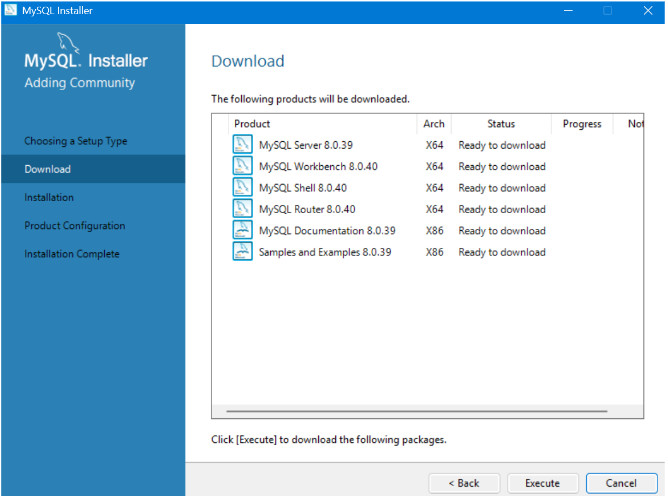
\includegraphics[width= 0.6\textwidth]{images/eexecute.png}
    \caption{Download MySQL}
\end{figure}

\subsection{Configurazione del account MySQL}
Una volta terminato il download, si procederà con la configurazione dell'account MySQL. Si dovrà quindi scegliere una password, necessaria per accedere al database. 


\begin{figure}[h!]
    \centering
    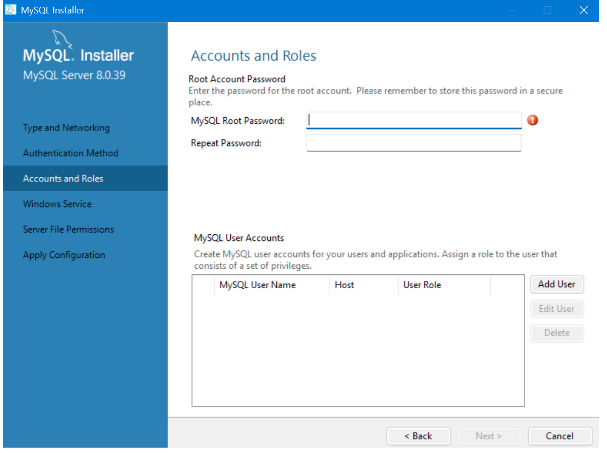
\includegraphics[width= 0.5\textwidth]{images/setup vero e proio musql.png}
    \caption{Configurazione account MySQL}
\end{figure}


Si giungerà infine alla scehermata di applicazione della configurazione del database. Cliccare su \textbf{Execute} per applicare la configurazione.

\begin{figure}[h!]
    \centering
    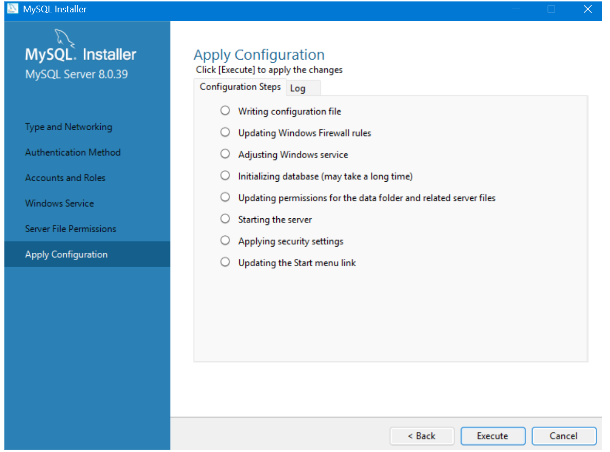
\includegraphics[width= 0.5\textwidth]{images/completamenot.png}
    \caption{Completamento installazione}
\end{figure}

Una volta terminata anche l'installazione del MySQL, si dovrà cliccare su \textbf{Finish} per chiudere l'installler. 

\begin{tcolorbox}[  colback=white!5!white, colframe=gray, title={Avvertenza} ]
    Per un corretto funzionamento sia del JDK che del MySQL, è consiglaito riavviare il computer.
    
\end{tcolorbox}


\subsection{Schermata finale}
Al termine dell'installazione il programma \texttt{resources.bat} mostrerà la seguente schermata. 

\begin{figure}[h!]
    \centering
    
\includegraphics[width= 0.6\textwidth]{images/insytllazione compeltata.png}
    \caption{Completamento installazione}
\end{figure}
